% 建议使用 XeLaTeX 或 LuaLaTeX 编译(中文与公式支持更佳)
\documentclass[UTF8,zihao=-4]{ctexart}

\usepackage[a4paper,margin=2.5cm]{geometry}
\usepackage{amsmath, amssymb, amsthm}
\usepackage{bm}
\usepackage{hyperref}
\usepackage{graphicx}
\usepackage{caption}
\usepackage{listings}
\usepackage{xcolor}
\usepackage{float}
\usepackage{placeins}
\graphicspath{{figures/}}

\lstdefinestyle{code}{
  basicstyle=\ttfamily\small,
  numbers=left,
  numberstyle=\tiny,
  numbersep=8pt,
  keywordstyle=\color{blue},
  commentstyle=\color{teal!70!black},
  stringstyle=\color{orange!70!black},
  showstringspaces=false,
  breaklines=true,
  frame=single,
  framerule=0.3pt,
  rulecolor=\color{black!15}
}
\lstset{style=code}

\title{策略梯度方法:原理、公式、应用与实战}
\author{}
\date{\today}

\begin{document}
\maketitle

\section{引言}
策略梯度(Policy Gradient)方法直接对参数化策略进行优化,通过梯度上升最大化期望回报。与依赖价值函数导出的策略不同,策略梯度天然支持连续动作空间、随机策略以及带约束的优化,是现代强化学习算法(如 PPO、TRPO)的一大基石。

\section{原理与公式}
\subsection{目标函数与策略梯度定理}
设随机策略 \(\pi_\theta(a\mid s)\) 由参数 \(\theta\) 控制,目标为折扣回报期望:
\begin{equation}
J(\theta) = \mathbb{E}_{\tau \sim \pi_\theta}\Big[ \sum_{t=0}^{T} \gamma^t r_{t+1} \Big].
\end{equation}
策略梯度定理给出:
\begin{equation}
\nabla_\theta J(\theta) = \mathbb{E}_{s \sim d^{\pi_\theta}, a \sim \pi_\theta}\big[ \nabla_\theta \log \pi_\theta(a\mid s)\, Q^{\pi_\theta}(s,a) \big],
\end{equation}
其中 \(d^{\pi_\theta}\) 为折扣状态分布。

\subsection{基线与优势函数}
为降低方差,可引入基线 \(b(s)\):
\begin{equation}
\nabla_\theta J(\theta) = \mathbb{E}\big[ \nabla_\theta \log \pi_\theta(a\mid s)\, (Q^{\pi}(s,a) - b(s)) \big].
\end{equation}
当 \(b(s)=V^{\pi}(s)\) 时即得到优势函数 \(A^{\pi}(s,a)\),引出 Actor-Critic 架构:策略(Actor)更新梯度,价值估计(Critic)提供基线。

\subsection{更新规则}
蒙特卡洛策略梯度(REINFORCE)执行随机梯度上升:
\begin{equation}
\theta_{k+1} = \theta_k + \alpha \sum_{t=0}^{T-1} \nabla_\theta \log \pi_{\theta_k}(a_t\mid s_t)\, \hat{A}_t,
\end{equation}
其中 \(\hat{A}_t\) 可用回报、广义优势估计等替代。梯度裁剪、熵正则以及自适应优化器(Adam)常用于稳定训练。

\section{应用与技巧}
\begin{itemize}
  \item \textbf{连续控制}:机器人、仿真控制与 locomotion 等连续动作任务。
  \item \textbf{约束优化}:在策略梯度框架下融入安全约束或成本惩罚。
  \item \textbf{模仿与微调}:以专家策略初始化,再通过策略梯度微调。
  \item \textbf{实用建议}:对优势值标准化,保持熵正则,使用自适应学习率,并监控梯度范数。
\end{itemize}

\section{Python 实战}
脚本 \texttt{gen\_policy\_gradient\_figures.py} 在随机 bandit 环境中训练 softmax 策略,使用 REINFORCE 搭配基线,记录每回合回报与梯度信息以展示收敛特性。
\begin{lstlisting}[language=Python,caption={脚本 gen_policy_gradient_figures.py 片段}]
grad = features[action] - (policy @ features)
baseline = baseline + baseline_lr * (G - baseline)
theta += alpha * grad * (G - baseline)
\end{lstlisting}

\section{实验结果}
\begin{figure}[H]
  \centering
  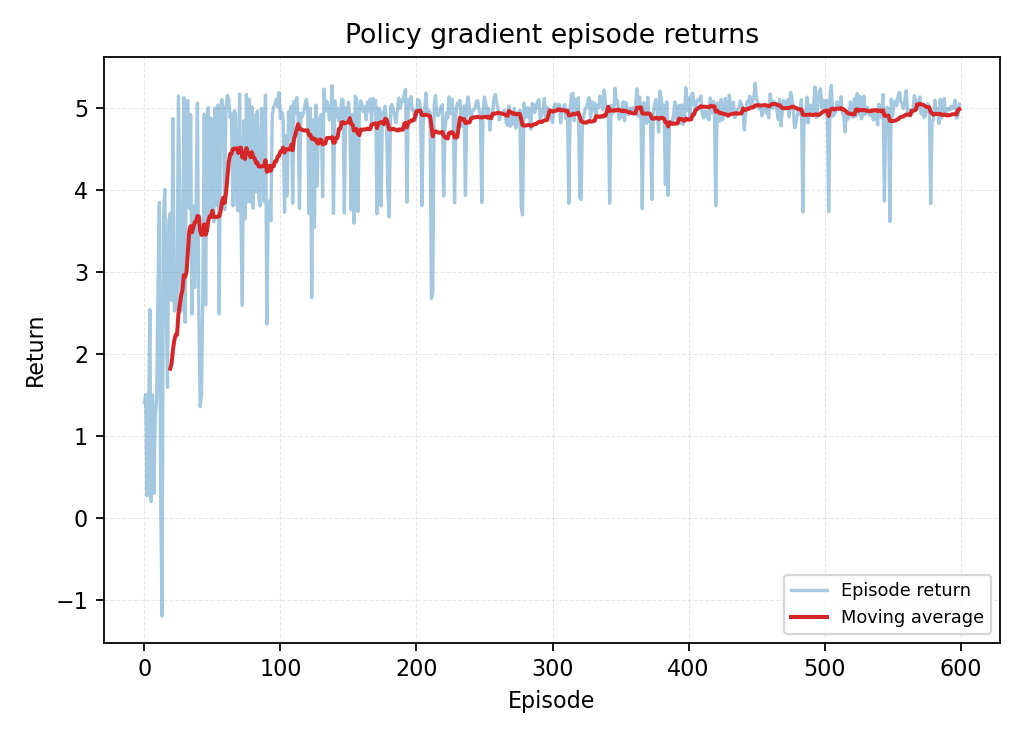
\includegraphics[width=0.8\linewidth]{policy_gradient_returns.png}
  \caption{策略梯度的回报曲线与滑动平均}
  \label{fig:policy_gradient_returns_cn}
\end{figure}

\begin{figure}[H]
  \centering
  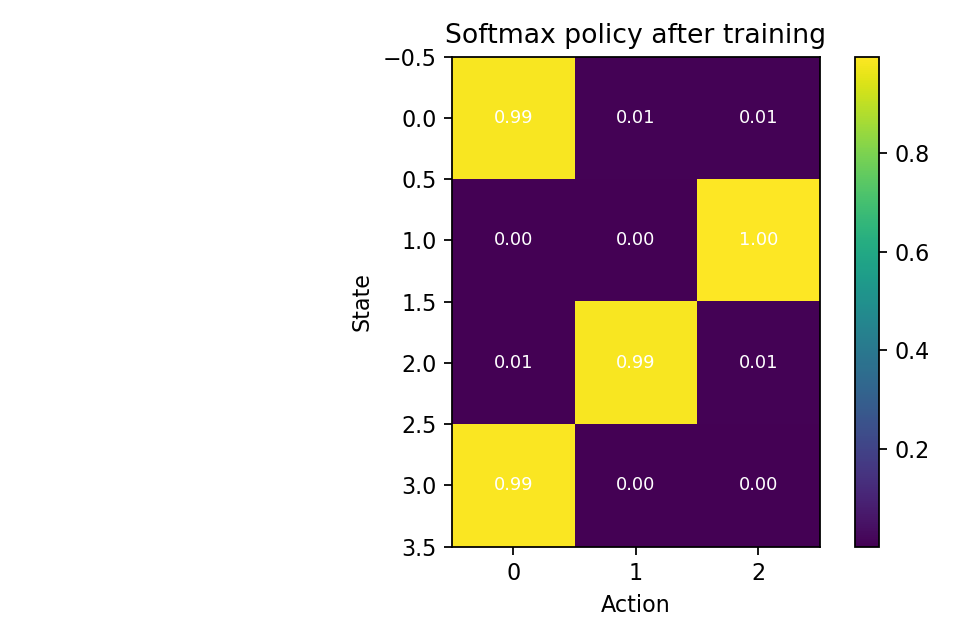
\includegraphics[width=0.82\linewidth]{policy_gradient_policy_heatmap.png}
  \caption{softmax 策略学得的状态-动作概率热力图}
  \label{fig:policy_gradient_policy_heatmap_cn}
\end{figure}

\FloatBarrier
\section{总结}
策略梯度通过对策略参数执行梯度上升,实现对期望回报的直接优化。合理的方差削减、熵正则与优化技巧是稳定训练的关键。示例展示了回报随训练提升以及策略分布如何向高回报动作倾斜。

\end{document}